
\chapter{基于渐进式策略的人体运动姿态预测算法}
本章节将围绕本文的两个主要贡献点:渐进式的网络学习框架和集成$SD-GCN$和$TD-GCN$的图卷积模块。分别从动机、方案、实现框架和算法细节几个方面对本方法进行详细的阐述。在此之前,我们首先通过数学语言定义人体运动姿态预测问题,并介绍在此过程中使用的相关数据结构,以方便在本文后续章节中进行准确的叙述。
\section{数据描述与问题定义}
\subsection{人体运动姿态数据结构}
\begin{figure}[ht]
    \centering
    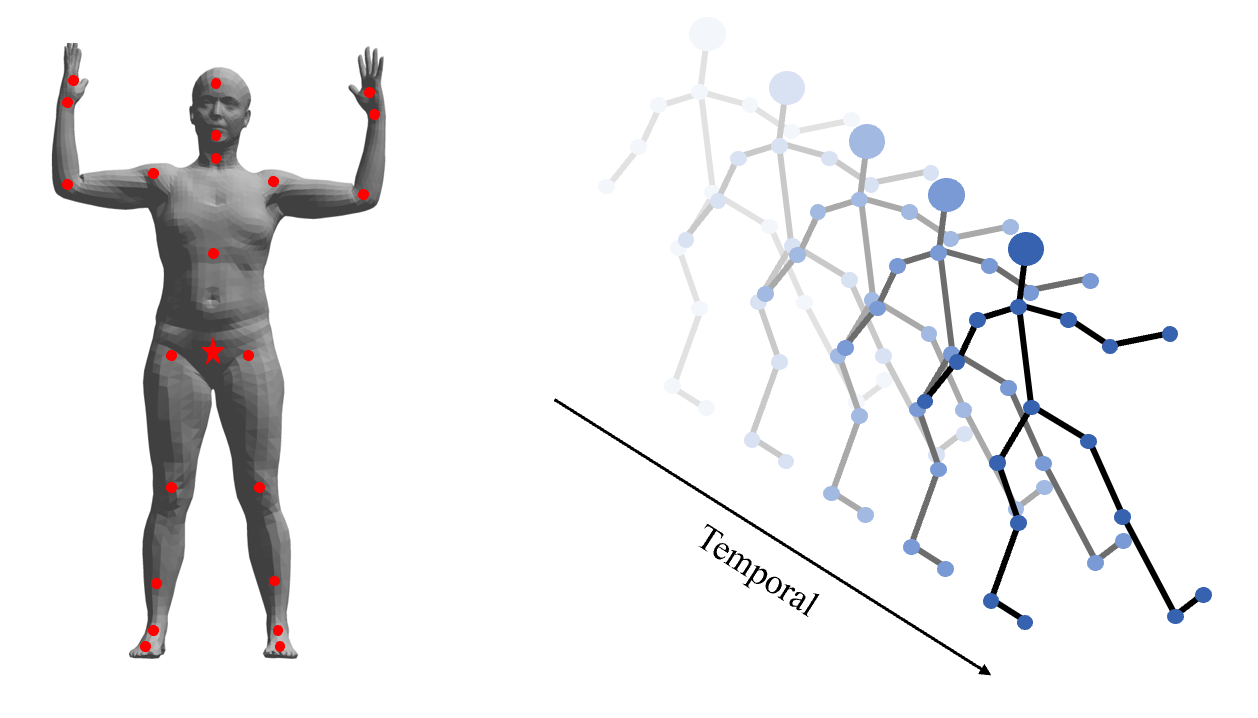
\includegraphics[width=0.85\textwidth]{FigMa/show_structure.png}\\
    \vspace{-0.3cm}
    \caption{人体运动姿态数据结构}
    \label{fig:data_structure}
\end{figure}
首先我们介绍人体运动姿态预测问题所使用的数据结构。如图\ref{fig:data_structure}左所示,人体运动数据是通过动作捕捉设备,在封闭室内或开放室外场景提取到的人体关键点运动数据,这些数据以SKT(Skeletal Kinematic Tree)的形式表示和存储。在实际动作捕捉过程中,通常只关注在运动过程中起决定性作用的关节点,例如手肘、肩部、膝盖等。这些关节点在\ref{fig:data_structure}左中以红色标记的形式展现。其中位于胯部的五角星节点被称为根节点,其余节点通过递归的形式计算自身对于根节点的相对位置来得到自身位置。由于本文仅关注三维欧式空间中的人体运动,因此,我们用与根节点的相对3D坐标来描述每个关节点空间位置。将独立的关节点按照人体结构连接后,即可得到抽象后人体姿态。由于我们处理的是序列数据,同时包含时间和空间两个维度的关节点,因此在\ref{fig:data_structure}右中,空间维度上描述人体结构信息,时间维度上描述关节点序列运动信息。

\subsection{人体运动姿态预测问题定义}
从数学上,对于一个长度为$T$的人体运动序列,我们将其定义为$S_{1:T} = \{P_1,P_2,\cdots,P_{T}\}$,其中$P_i$当前运动序列中位于$i$时刻的人体姿态。每个人体姿态$P_i$又由若干个关节点组成其中$P \in \mathbb{R}^N$,$N$为该人体姿态包含的关节点数量。

对于人体运动姿态预测问题,网络$\Phi$接收已知输入序列$S_{1:T_h} = \{P_1,P_2,\cdots,P_{T_h}\}$作为输入,预测未来运动序列$S_{T_h+1:T_h+T_f} = \{P_{T_h+1},P_{T_h+2},\cdots,P_{T_h+T_f}\}$,这一过程的数学描述如公式\ref{equation:problem_formulation}所示。其中$\theta$为可训练的网络参数。
\begin{equation}
    S_{T_h+1:T_h+T_f} = \Phi(S_{1:T_h}, \theta) \label{equation:problem_formulation}
\end{equation}

\section{渐进式人体运动序列预测框架}
正如\ref{section:1.1}节所提到的,预测过程中的不确定性是影响预测精确度进一步提升的关键因素,而这种不确定性来自输入运动序列和待预测序列之间的差异。简而言之,由于输入运动序列和预测运动序列之间存在较大差异(例如,输入运动和待预测运动的运动模式有较大差异),网络无法根据输入序列中的信息来准确推测未来运动,导致预测结果脱离真实情况。因此,如何降低预测过程中的不确定性成为了当务之急。

在调研过程中,我们注意到LTD\parencite{mao2019learning}提出的一项改进使得预测精度相较于现有方法得到了极大提升。在早期的方法中,如公式\ref{equation:problem_formulation}所示,输入运动序列长度$1:T_h$与预测序列长度$T_h+1:T_h+T_f$通常存在差异,通常预测序列的长度要远远长于输入序列(例如,输入10帧预测25帧),这使得网络需要在毫无参考基础的情况下去构造未来运动序列。这通常会导致预测结果不连续,与真值出现较大偏差。针对该现象,LTD\parencite{mao2019learning}提出公式\ref{equation:padding},通过使用输入序列的最后一帧来填充输入序列,使得输入序列的长度和预测序列保持一致。
\begin{equation}
    \begin{aligned}
        &\widetilde{S}_{1:T_h} = [S_{1:T_h}, \{P^{T_h+1}_{T_h}, \cdots, P^{T_f}_{T_h} \} ]
        \\
        &S_{T_h+1:T_h+T_f} = \Phi(\widetilde{S}_{1:T_h}, \theta)
    \end{aligned}
    \label{equation:padding}
\end{equation}

从图\ref{fig:LTD_padding}可以看到,经过填充后的输入数据对网络有两点促进作用,第一,输入和输出维度一致,避免了数据维度变换过程中的不确定性。第二,网络在预测未来序列时可以在已知部分最后一帧基础上进行预测,降低了预测的难度。
\begin{figure}[ht]
    \centering
    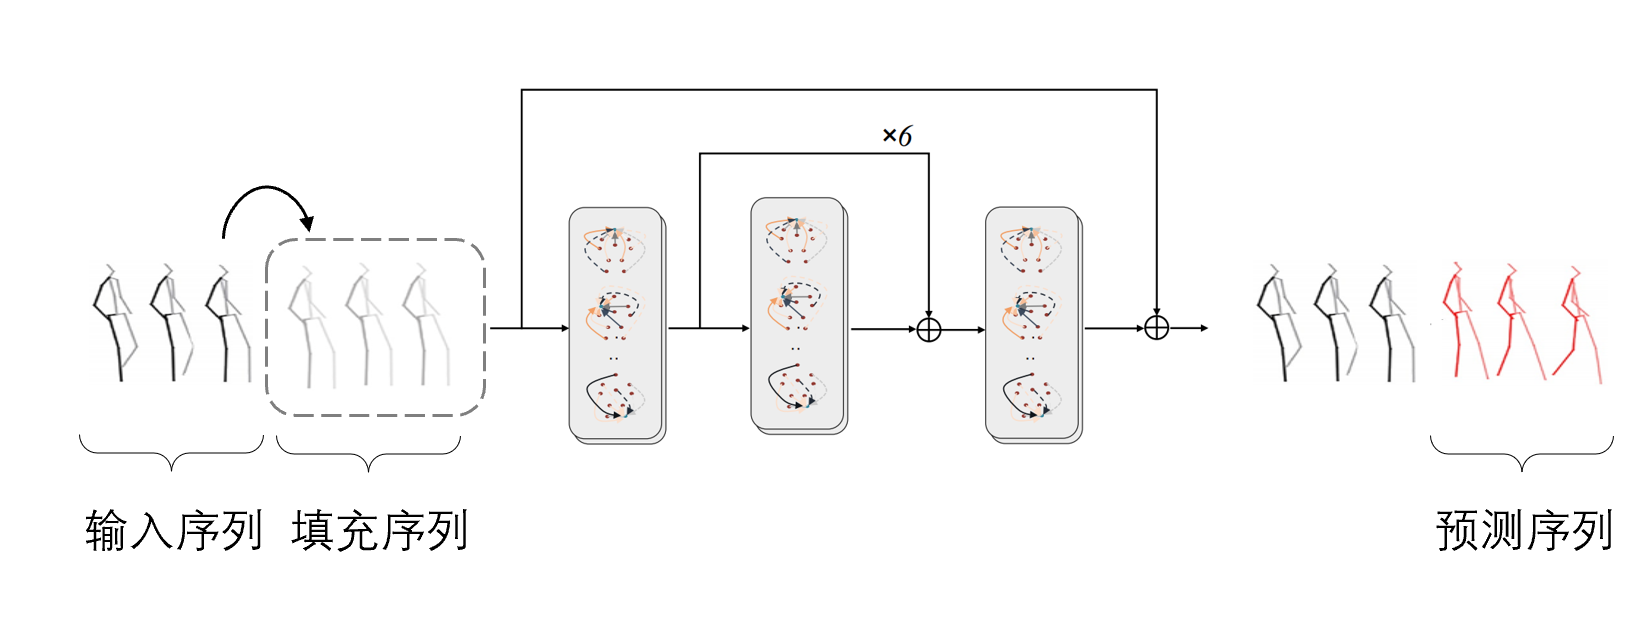
\includegraphics[width=1\textwidth]{FigMa/LTD_padding.png}\\
    \vspace{-0.3cm}
    \caption{LTD数据填充过程}
    \label{fig:LTD_padding}
\end{figure}
然而这种粗糙的填补方法也有其固有缺陷。首先整个填充过程不区分时序距离,全部使用最后一帧进行填充,对于离$P_{T_h}$较近的未来运动,$P_{T_h}$还能提供一定的参考。随着时间向前,未来帧与$P_{T_h}$的关联越来越弱,其提供的参考价值也越来越低,预测的不确定性也逐渐增加。因此该填充方法无法缓解较远距离的预测不确定问题。

在分析上述方法得失后,我们认为,缩小输入序列和待预测序列的差异(维度差异、内容差异等)可以有效降低预测过程中的不确定性,使得预测结果向我们期望的方向趋近。但单纯地填充输入序列最后一帧所带来的性能提升还有一定的上涨空间。如何为预测过程提更高效的预测基础将是需要重点考虑的问题。

受到最近被广泛应用的由粗糙到精细(Coarse To Fine)策略的启发,我们设计了一个简易实验来验证我们的想法。Coarse to fine 策略与大多数一步到位的方法不同,预测被分为了两个阶段。位于网络浅层的阶段被称为粗糙(Coarse)网络,它接收原始的输入,并输出一个较为粗糙的结果,虽然该结果离最终的目标存在一定的偏差,但与最初的输入信息相比,它已经包含了目标的绝大部分信息。随后该粗糙结果被送入精修(Fine)网络,精修网络将在粗糙网络的基础上进一步完善预测细节。该策略被广泛应用于图片修复(Image Inpainting)\parencite{yu2018generative,zamir2021multi}领域,原始缺失图片通常由粗糙网络生成一个低分辨率较模糊的修复版本,此次修复的目的是修复图片内容的结构。随后,粗修版本被送入精修网络提高分辨率并进一步完善细节,最后输出高质量的修复结果。参考该思路,我们设计了一个Coarse To Fine 人体运动序列预测网络。

\begin{figure}[ht]
    \centering
    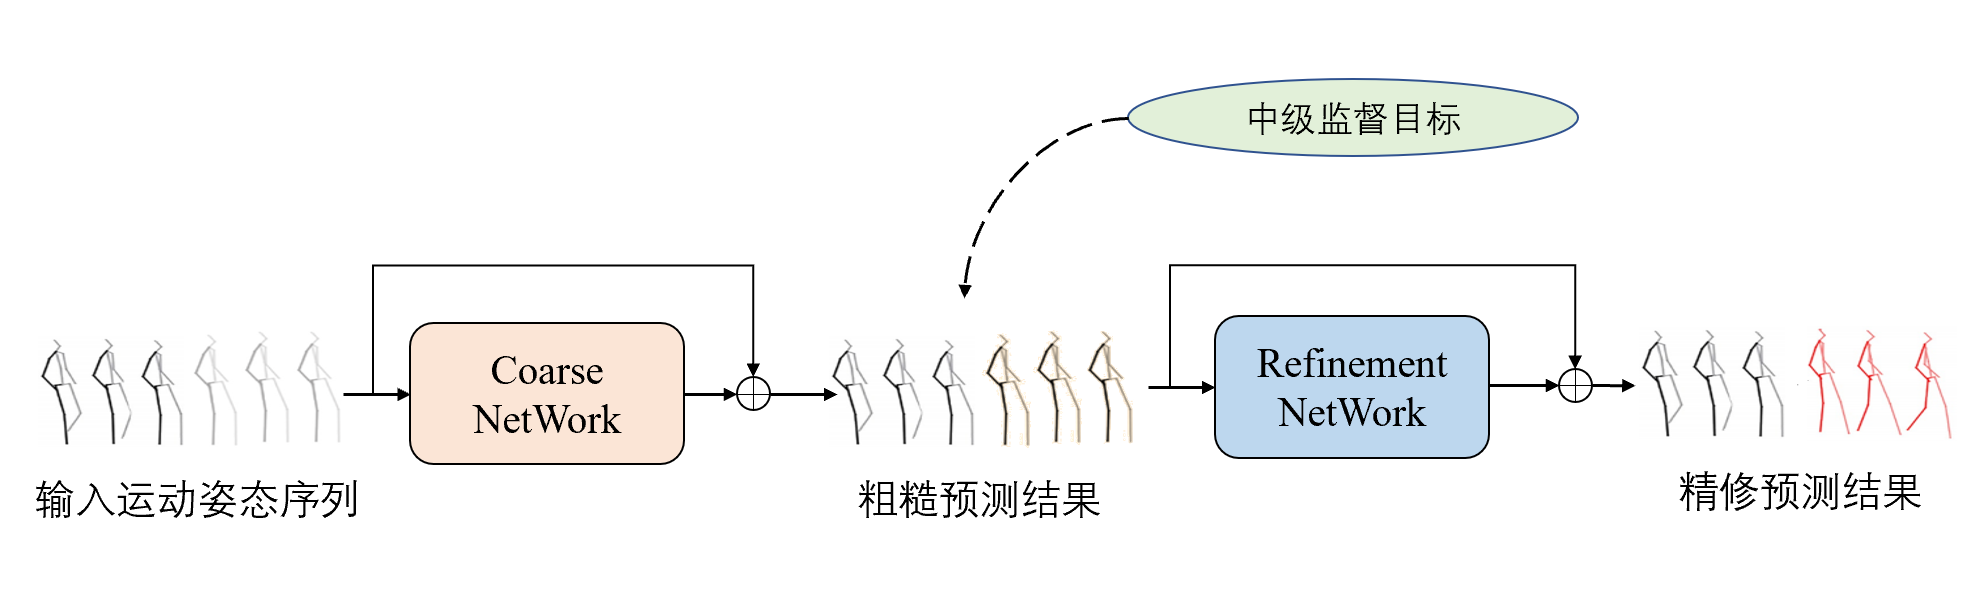
\includegraphics[width=0.9\textwidth]{FigMa/Two_stage.png}\\
    \vspace{-0.3cm}
    \caption{Coarse To Fine 预测网络}
    \label{fig:Two_stage}
\end{figure}